\subsection{Silent edges}
\begin{frame}{Silent edges}
\label{sec:unobservable}
\begin{columns}
\begin{column}{0.5\textwidth}

\only<1| handout:1>{
Edges silent in RNA logFC data simulated on arbitrary graph

% When inferring a protein-protein or protein-DNA interaction using RNA log fold-change values it is a basic assumption that the RNA values will be affected by the presence or absence of said interaction. In a graph model a TF edge will be observable if the target of the edge is a gene directly measured in the RNA log fold-change data.

% The protein kinases can have outgoing edges with TFs or other PKs as target~(\autoref{fig:unobservable}). If the target of their edge is a TF, then the PK edge will only be detectable if the same can be said for at least one edge from the TF to a measured gene. If the target of the PK edge is another PK, then in order to be detectable, the target will have to have at least one detectable outgoing edge. 


% For real data we will assume that enough genes are recorded that any direct protein-protein or protein-DNA interaction should have some level of effect on gene expression, however small, and that kinase regulation has an effect on gene expression. It is more relevant to consider undetectability for graphs designed artificially from more-or-less random adjacency matrices where it can occur that edges lead to nodes having no outgoing edges themselves.

% A nonsilent node is a node with at least one nonsilent outgoing edge. From a graph with known adjacency matrix $W$ we calculate which nodes are nonsilent with

\begin{equation}
\label{eq:detectable}
\boldsymbol{\omega} =
\sign \sum_{k=0}^K {|W|^\trans}^k
I_T |W|^\trans \boldsymbol{1} 
\end{equation}
\begin{conditions}
|W| & element-wise absolute of $W$ \\
\boldsymbol{1} & vector of 1s
\end{conditions}
% Here $\boldsymbol{\omega}$ is a vector where entry $\omega_i$ will be 1 if node $i$ is detectable and 0 otherwise. The superscript $\trans$ refers to transposing. $W$ has to be square, which it is in all cases where this equation has been applied. $\sign$ is the sign function, $|W|$ is the absolute of $W$, $\boldsymbol{1}$ is a vector of 1s with length $N_T + N_P$. $K$ is the length of the longest cascade of protein kinases, which is found through iterative calculation of $\boldsymbol{\omega}(K)$ as the smallest $K$ for which it holds that $\boldsymbol{\omega}(K) = \boldsymbol{\omega}(K + 1)$.


% \autoref{eq:detectable} can be read as starting with finding all TFs with at least one outgoing edges~($W^\trans \boldsymbol{1} I_T$), and iteratively follow all kinase cascades backwards for each iteration $k$.
}

\only<2| handout:2>{

% The simple network in~\autoref{fig:unobservable} can be used as an example, where we assign some random positive and negative values to each edge. Columns and rows in $W$ are sorted with TF first and PK second, so the order is $\text{TF}_1,\text{TF}_2,\text{TF}_3,\text{PK}_1,\text{PK}_2,\text{PK}_3$.

\begin{subequations}
\begin{align*}
\label{eq:detectable_example}
W &=
\begin{bmatrix} 
0 & 0 & 0 & 0 & 0 & -0.8 \\
0 & 0 & 0 & 0 & 0 & 0.7 \\
0 & 0 & 0 & 0 & -0.1 & 0.3 \\
1.1 & 0 & 0 & 0 & 0 & -0.4 \\
0 & 0 & 0 & 0 & 0 & 0 \\
0 & 0 & 0 & 0 & 0.5 & 0 \\
\end{bmatrix}
\\
|W|^\trans &=
\begin{bmatrix} 
0 & 0 & 0 & 1.1 & 0 & 0 \\
0 & 0 & 0 & 0 & 0 & 0 \\
0 & 0 & 0 & 0 & 0 & 0 \\
0 & 0 & 0 & 0 & 0 & 0 \\
0 & 0 & 0.1 & 0 & 0 & 0.5 \\
0.8 & 0.7 & 0.3 & 0.4 & 0 & 0 \\
\end{bmatrix}
\end{align*}
\end{subequations}

}


\only<3| handout:3>{

\begin{subequations}
\begin{align*}
I_T |W|^\trans \boldsymbol{1}
=
\sum_{k=0}^0 {|W|^\trans}^k
I_T |W|^\trans \boldsymbol{1}
&=
\begin{bmatrix} 
1.1 \\
0 \\
0 \\
0 \\
0 \\
0 \\
\end{bmatrix}
\\
\sum_{k=0}^1 {|W|^\trans}^k
I_T |W|^\trans \boldsymbol{1}
&=
\begin{bmatrix} 
1.1 \\
0 \\
0 \\
0 \\
0 \\
0.88 \\
\end{bmatrix}
\end{align*}
\end{subequations}

}

\only<4| handout:4>{

\begin{subequations}
\begin{align*}
\sum_{k=0}^2 {|W|^\trans}^k
I_T |W|^\trans \boldsymbol{1}
&=
\begin{bmatrix} 
1.1 \\
0 \\
0 \\
0 \\
0.44 \\
0.88 \\
\end{bmatrix}
\\
\sum_{k=0}^3 {|W|^\trans}^k
I_T |W|^\trans \boldsymbol{1}
&=
\begin{bmatrix} 
1.1 \\
0 \\
0 \\
0 \\
0.44 \\
0.88 \\
\end{bmatrix}
\end{align*}
\end{subequations}
}
\only<5| handout:5>{
% There is no change in the calculation from $K=2$ to $K=3$ so we set $K$ equal to 2 and get
\begin{equation*}
\label{eq:silent_example}
\boldsymbol{\omega} = \begin{bmatrix} 
1 \\
0 \\
0 \\
0 \\
1 \\
1 \\
\end{bmatrix}
\quad,\quad
M_s =
\begin{bmatrix} 
1 & 1 & 1 & 1 & 1 & 1 \\
1 & 1 & 1 & 0 & 0 & 0 \\
1 & 1 & 1 & 0 & 0 & 0 \\
1 & 1 & 1 & 0 & 0 & 0 \\
1 & 1 & 1 & 1 & 1 & 1 \\
1 & 1 & 1 & 1 & 1 & 1 \\
\end{bmatrix}
\end{equation*}
% This means that $\text{TF}_2,\text{TF}_3,\text{PK}_1$ are silent nodes. From $\boldsymbol{\omega}$ we can find the set of silent edges, which are all activity regulating edges onto any of the silent nodes. These entries in $W$ of silent edge is shown as zeros in $M_S$~(\autoref{eq:silent_example}), which is the masking matrix that indicates the edges to consider for a performance evaluation on an edge inference attempt. It is clear to spot the four edges in $W$ that are too be ignored if we were to infer edges for this network.
}
\stepcounter{equation}
\end{column}
\begin{column}{0.5\textwidth}
\begin{figure}[ht]
    \centering
    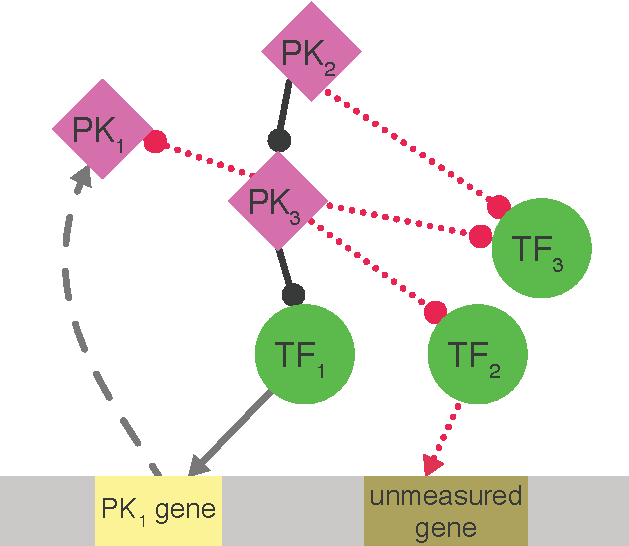
\includegraphics[width=0.6\textwidth]{theory/fig/unobservable.pdf}
    \caption{\textbf{Silent edges.} \textcolor{red}{red} = silent, \textcolor{black}{black} = detectable PK edge, dashed = transcription/translation, \textcolor{darkgray}{dark gray} = TF edge. }
    \label{fig:unobservable}
\end{figure}

\end{column}
\end{columns}
\end{frame}

\begin{frame}{Silent edges - removing $K$}
% As mentioned, $K$ in~\autoref{eq:detectable} is the length of the longest kinase cascade, or more precisely, the iteration where, if we computed further iterations of the sum, it would not change $\boldsymbol{\omega}$. We can simplify by letting $K$ tend to infinity.
for $K\rightarrow\infty$
\begin{equation}
\boldsymbol{\omega} =
\sign \sum_{k=0}^\infty {|W|^\trans}^k
I_T |W|^\trans \boldsymbol{1}
=
\sign \left( \left( \sum_{k=0}^\infty {|W|^\trans}^k \right)
I_T |W|^\trans \boldsymbol{1} \right)
\end{equation}
% If $I-|W|^\trans$ is invertible we can simplify the sum, using the same rule applied by Eberhardt~et~al.~(\autoref{eq:eber_converge.b}). We assume this holds since our system~(\autoref{eq:basic_eberhardt_extension}) is meant to reach equilibrium. It will not be assumed to hold for "gold standard" matrices discussed later~(\autoref{sec:dream_data}), since these does not hold edge values before preprocessing, and would diverge if used as such.
Simplify using same rule applied by Eberhardt~et~al.~(eq.~\ref{eq:eber_converge})
\begin{equation}
\label{eq:detectable_no_K}
\boldsymbol{\omega} =
\sign \left( \left( I - {|W|^\trans} \right)^{-1}
I_T |W|^\trans \boldsymbol{1} \right)
\end{equation}
% \autoref{eq:detectable_no_K} was tested on $W$ given in \autoref{eq:detectable_example}, which as expected produced $\boldsymbol{\omega}$ from \autoref{eq:silent_example} (a tolerance of $>\num{1e-14}$ was used instead of $\sign$ due to the imperfect nature of floating-point computation).
\end{frame}